\documentclass[tikz,border=2pt]{standalone}
\usepackage{amsmath,amssymb}
\usetikzlibrary{arrows.meta}
\begin{document}
% Same five-job path as on the arrival-average page: the area under L(t) on [0,9] is
% sum of sojourn times = 10 job-minutes; the time average 10/9 (green dashed) has equal area.
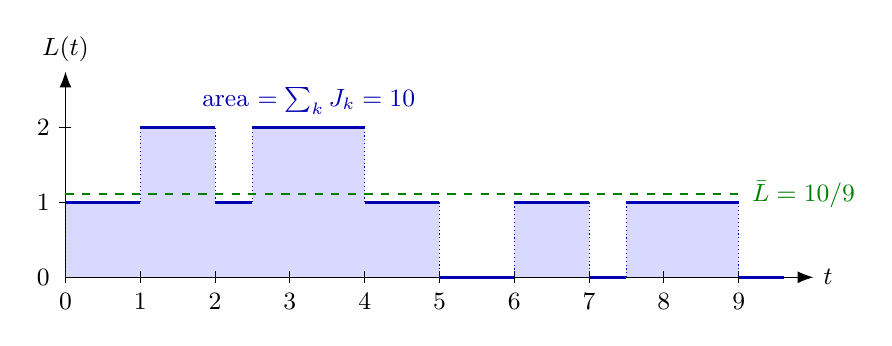
\begin{tikzpicture}[font=\small, >={Latex[length=2mm]}, x=0.95cm, y=0.95cm]
  % shaded area under the path
  \fill[blue!15] (0,0) -- (0,1) -- (1,1) -- (1,2) -- (2,2) -- (2,1) -- (2.5,1) -- (2.5,2)
    -- (4,2) -- (4,1) -- (5,1) -- (5,0) -- (6,0) -- (6,1) -- (7,1) -- (7,0) -- (7.5,0)
    -- (7.5,1) -- (9,1) -- (9,0) -- cycle;
  % axes
  \draw[->] (0,0) -- (10,0) node[right] {$t$};
  \draw[->] (0,0) -- (0,2.75) node[above] {$L(t)$};
  \foreach \y in {1,2} {\draw (0.08,\y) -- (-0.08,\y) node[left] {$\y$};}
  \node[left] at (-0.08,0) {$0$};
  \foreach \x in {0,1,2,...,9} {\draw (\x,0.08) -- (\x,-0.08) node[below] {$\x$};}
  % sample path
  \draw[blue!70!black, very thick]
    (0,1) -- (1,1) (1,2) -- (2,2) (2,1) -- (2.5,1) (2.5,2) -- (4,2)
    (4,1) -- (5,1) (5,0) -- (6,0) (6,1) -- (7,1) (7,0) -- (7.5,0)
    (7.5,1) -- (9,1) (9,0) -- (9.6,0);
  \foreach \x/\a/\b in {0/0/1, 1/1/2, 2/2/1, 2.5/1/2, 4/2/1, 5/1/0, 6/0/1, 7/1/0, 7.5/0/1, 9/1/0}
    {\draw[blue!70!black, thin, densely dotted] (\x,\a) -- (\x,\b);}
  % time average
  \draw[green!50!black, thick, dashed] (0,10/9) -- (9,10/9);
  \node[green!50!black, anchor=west] at (9.05,10/9) {$\bar L=10/9$};
  % area label
  \node[blue!70!black, anchor=south] at (3.25,2.05) {area $=\sum_k J_k=10$};
\end{tikzpicture}
\end{document}
